\documentclass{standalone}

\usepackage{tikz}
\usetikzlibrary{arrows,calc,shapes}

\renewcommand{\familydefault}{\sfdefault}

\tikzstyle{block} = [draw,rounded corners,fill=blue!20,inner sep=0pt]
\tikzstyle{io-block} = [draw,rounded corners,fill=red!20,inner sep=0pt]
\tikzstyle{mixer} = [regular polygon, regular polygon sides=3,draw, fill=blue!20, text width=1em,inner sep=1mm, outer sep=0mm, shape border rotate=-90]

\begin{document}

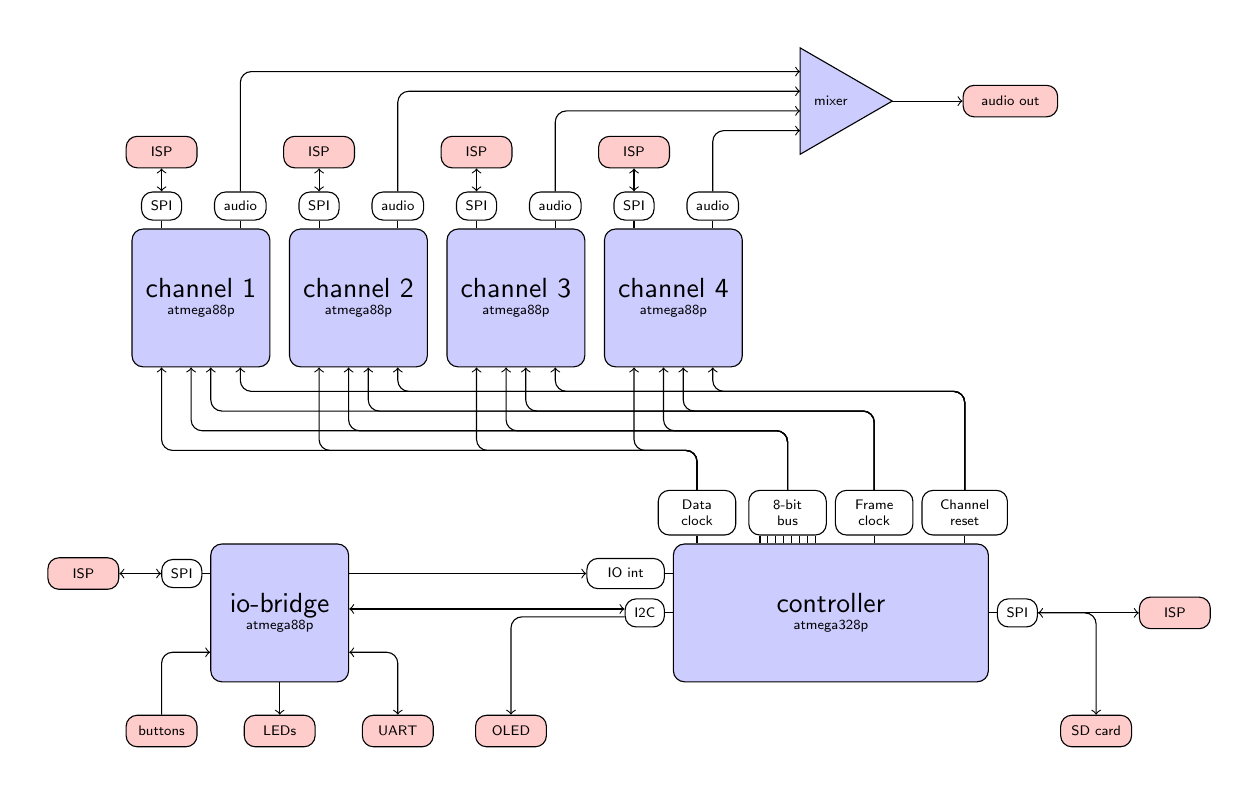
\begin{tikzpicture}
%  \draw (-10,-1.75) rectangle (4.9,7.2);
  
  \node [block,minimum width=4cm,minimum height=1.75cm] (controller) at (0,0) {\parbox{1.4cm}{\centering controller \\ \tiny atmega328p}};
  \node [block,minimum width=1.75cm,minimum height=1.75cm] (io-bridge) at (-7,0) {\parbox{1.4cm}{\centering io-bridge \\ \tiny atmega88p}};

  \node [block,minimum width=1.75cm,minimum height=1.75cm] (channel-1) at (-8,4) {\parbox{1.75cm}{\centering channel 1 \\ \tiny atmega88p}};
  \node [block,minimum width=1.75cm,minimum height=1.75cm] (channel-2) at (-6,4) {\parbox{1.75cm}{\centering channel 2 \\ \tiny atmega88p}};
  \node [block,minimum width=1.75cm,minimum height=1.75cm] (channel-3) at (-4,4) {\parbox{1.75cm}{\centering channel 3 \\ \tiny atmega88p}};
  \node [block,minimum width=1.75cm,minimum height=1.75cm] (channel-4) at (-2,4) {\parbox{1.75cm}{\centering channel 4 \\ \tiny atmega88p}};

  \node [io-block,minimum width=0.9cm,minimum height=0.4cm] (OLED) at ($(controller.west)!0.5!(io-bridge.east)-(0,1.5)$) {\tiny OLED};
  \node [io-block,minimum width=0.9cm,minimum height=0.4cm] (UART) at ($(io-bridge)+(1.5,-1.5)$) {\tiny UART};
  \node [io-block,minimum width=0.9cm,minimum height=0.4cm] (LEDs) at ($(io-bridge)+(0,-1.5)$) {\tiny LEDs};
  \node [io-block,minimum width=0.9cm,minimum height=0.4cm] (buttons) at ($(io-bridge)+(-1.5,-1.5)$) {\tiny buttons};

  \coordinate (controller-i2c-c) at (controller.west);
  \coordinate (controller-spi-c) at (controller.east);
  \coordinate (controller-bus-c) at ($(controller.north)+(-0.55,0)$);
  \coordinate (controller-dclk-c) at ($(controller.north)+(-1.7,0)$);
  \coordinate (controller-fclk-c) at ($(controller.north)+(+0.55,0)$);
  \coordinate (controller-ch-res-c) at ($(controller.north)+(+1.7,0)$);
  \coordinate (controller-io-int-c) at ($(controller.west)+(0,0.5)$);

  \coordinate (io-bridge-spi-c) at ($(io-bridge.west)+(0,0.5)$);
  \coordinate (io-bridge-buttons-c) at ($(io-bridge.west)-(0,0.5)$);
  \coordinate (io-bridge-UART-c) at ($(io-bridge.east)-(0,0.5)$);
  \coordinate (io-bridge-LEDs-c) at (io-bridge.south);
  \coordinate (io-bridge-io-int-c) at ($(io-bridge.east)+(0,0.5)$);


  \node [mixer] (mixer) at (0,6.5) {};
  \node at ($(mixer)-(0,0)$) {\tiny mixer};

  \coordinate (audio-out-1) at ($(mixer.west)+(0,0.375)$);
  \coordinate (audio-out-2) at ($(mixer.west)+(0,0.125)$);
  \coordinate (audio-out-3) at ($(mixer.west)-(0,0.125)$);
  \coordinate (audio-out-4) at ($(mixer.west)-(0,0.375)$);


  \foreach \n in {1,2,3,4} {
    \coordinate (channel-\n-dclk) at ($(channel-\n.south)+(-0.5,0)$);
    \coordinate (channel-\n-bus) at ($(channel-\n.south)+(-0.125,0)$);
    \coordinate (channel-\n-fclk) at ($(channel-\n.south)+(+0.125,0)$);
    \coordinate (channel-\n-reset) at ($(channel-\n.south)+(+0.5,0)$);

    \coordinate (channel-\n-spi-c) at ($(channel-\n.north)+(-0.5,0)$);
    \coordinate (channel-\n-audio-c) at ($(channel-\n.north)+(+0.5,0)$);

    \node (channel-\n-spi) at ($(channel-\n-spi-c)+(0,0.1)$) [draw,rounded corners,anchor=south] {\tiny SPI};
    \node (channel-\n-audio) at ($(channel-\n-audio-c)+(0,0.1)$) [draw,rounded corners,anchor=south] {\tiny audio};

    \draw (channel-\n-spi-c) -- (channel-\n-spi);
    \draw (channel-\n-audio-c) -- (channel-\n-audio);

    \node [io-block,minimum width=0.9cm,minimum height=0.4cm] (channel-\n-ISP) at ($(channel-\n-spi.north)+(0,0.5)$) {\tiny ISP};
    \draw [<->] (channel-\n-spi) -- (channel-\n-ISP);

    \draw [rounded corners,->] (channel-\n-audio) |- (audio-out-\n);
  }

  \node [io-block,minimum width=1.2cm,minimum height=0.4cm] (audio-out) at ($(mixer.east)+(1.5,0)$) {\tiny audio out};

  \draw [->] (mixer.east) -- (audio-out);


  \node (controller-i2c) at ($(controller-i2c-c)+(-0.1,0)$) [draw,rounded corners,anchor=east] {\tiny I2C};
  \node (controller-spi) at ($(controller-spi-c)+(+0.1,0)$) [draw,rounded corners,anchor=west] {\tiny SPI};

  \node [io-block,minimum width=0.9cm,minimum height=0.4cm] (SD-card) at ($(controller-spi)+(1,-1.5)$) {\tiny SD card};
  \node [io-block,minimum width=0.9cm,minimum height=0.4cm] (controller-ISP) at ($(controller-spi)+(2,0)$) {\tiny ISP};

  \node (io-bridge-spi) at ($(io-bridge-spi-c)+(-0.1,0)$) [draw,rounded corners,anchor=east] {\tiny SPI};

  \node [io-block,minimum width=0.9cm,minimum height=0.4cm] (io-bridge-ISP) at ($(io-bridge-spi)-(1.25,0)$) {\tiny ISP};
  
  \node (controller-bus) at ($(controller-bus-c)+(0,0.1)$) [draw,rounded corners,anchor=south] {\parbox{0.75cm}{\centering \tiny 8-bit \\ bus}};
  \node (controller-dclk) at ($(controller-dclk-c)+(0,0.1)$) [draw,rounded corners,anchor=south] {\parbox{0.75cm}{\centering \tiny Data \\ clock}};
  \node (controller-fclk) at ($(controller-fclk-c)+(0,0.1)$) [draw,rounded corners,anchor=south] {\parbox{0.75cm}{\centering \tiny Frame \\ clock}};
  \node (controller-ch-res) at ($(controller-ch-res-c)+(0,0.1)$) [draw,rounded corners,anchor=south] {\parbox{0.85cm}{\centering \tiny Channel \\ reset}};
  \node (controller-io-int) at ($(controller-io-int-c)-(0.1,0)$) [draw,rounded corners,anchor=east] {\parbox{0.75cm}{\centering \tiny IO int}};


  \draw (controller-spi-c) -- (controller-spi);
  \draw (controller-i2c-c) -- (controller-i2c);
  \draw (controller-dclk-c) -- (controller-dclk);
  \draw (controller-fclk-c) -- (controller-fclk);
  \draw (controller-ch-res-c) -- (controller-ch-res);
  \draw (controller-io-int-c) -- (controller-io-int);

  \draw [->] (io-bridge-io-int-c) -- (controller-io-int);

  \draw (io-bridge-spi-c) -- (io-bridge-spi);

  \foreach \x in {-0.35, -0.25, -0.15, -0.05, 0.05, 0.15, 0.25, 0.35} {
    \draw ($(controller-bus-c)+(\x,0)$) -- ($(controller-bus.south)+(\x,0)$);
  }
  
  \draw [<->] ($(controller-i2c.west)+(0,0.05)$) -- ($(io-bridge.east)+(0,0.05)$);
  \draw [rounded corners,->] ($(controller-i2c.west)-(0,0.05)$) -| (OLED.north);

  \draw [rounded corners,<->] (controller-spi.east) -| (SD-card.north);
  \draw [rounded corners,->] (controller-spi.east) -- (controller-ISP.west);

  \draw [rounded corners,<->] (io-bridge-spi.west) -- (io-bridge-ISP.east);

  \draw [rounded corners,<->] (io-bridge-UART-c) -| (UART);
  \draw [rounded corners,->] (io-bridge-LEDs-c) -- (LEDs);
  \draw [rounded corners,<-] (io-bridge-buttons-c) -| (buttons);

  \foreach \n in {1,2,3,4} {
    \draw [rounded corners,->] (controller-dclk.north) -- ($(controller-dclk.north)+(0,0.5)$) -| (channel-\n-dclk);
    \draw [rounded corners,->] (controller-bus.north) -- ($(controller-bus.north)+(0,0.75)$) -| (channel-\n-bus);
    \draw [rounded corners,->] (controller-fclk.north) -- ($(controller-fclk.north)+(0,1)$) -| (channel-\n-fclk);
    \draw [rounded corners,->] (controller-ch-res.north) -- ($(controller-ch-res.north)+(0,1.25)$) -| (channel-\n-reset);
  }

  \coordinate (sw) at (current bounding box.south west);
  \coordinate (ne) at (current bounding box.north east);
  
  \useasboundingbox ($(sw)-(0.25,0.25)$) rectangle ($(ne)+(0.25,0.25)$);
  
\end{tikzpicture}

\end{document}
